%! Author = Tom
%! Date = 07.12.2022
\chapter{Einleitung}

In diesem Kapitel führen wir an das Thema heran und stellen unsere Motive dar.
Wir definieren, welche Ziele wir in dieser Arbeit verfolgen und geben abschließend eine grobe Übersicht über die
Kapitelstruktur.

\section{Motivation}

Mit einer steigenden Nutzung von GraphQL wird es immer wichtiger, Tests für GraphQL-APIs zu entwickeln damit eine
gute Softwarequalität sichergestellt werden kann.
Die Entwicklung von Tests kann manuell oder automatisch geschehen.
Bei Unit-Tests, also Tests für einzelne Funktionen, kann ein Programmierer selbst entscheiden, ob er diese selbst schreiben will
oder von einem Tool automatisch generieren lasen will.
Integrations-Tests, also Tests die Kombinationen einzelner Interaktionen von Funktionen miteinander testen, hingegen haben sehr oft
einen sehr großen Testraum, sodass ein manuelles Schreiben dieser Tests fehleranfällig und langwierig ist.
Für REST-APIs existieren schon automatische Integrationstesttools wie zum Beispiel: EvoMaster \cite{evo-master} , QuickREST \cite{karlsson2019quickrest} oder RESTTESTGEN \cite{rest-test-gen}.
GraphQL-APIs haben leider noch einen Mangel an solchen automatischen Testtools.
Im Rahmen der internationalen  Konferenz für Automatisierung  von  Softwaretests IEEE/ACM 2021 wurde mit
\textit{Automatic Property-based Testing of GraphQL APIs}\cite{property-based-testing} eine Methode vorgestellt, die diesen Mangel angehen soll.
Es wurde eine Methode entwickelt die aus dem GraphQL-Schema, also der Beschreibung der Datenstruktur der API, Tests zufällig generiert und damit versucht Fehler in der Programmierung zu finden.
Die entwickelte Methode arbeitet nach dem in Abbildung~\ref{property-based-method} gezeigten Prinzip.

\begin{figure}[h!]
    \centering
    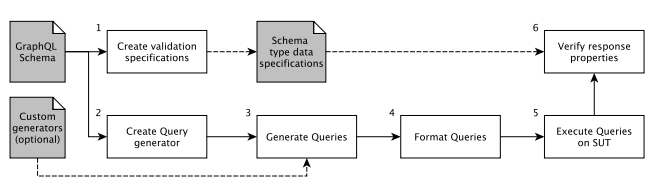
\includegraphics[width=\textwidth,height=\textheight,keepaspectratio]{content/einleitung/toolchain}
    \caption{Methode von~\cite{property-based-testing}}
    \label{property-based-method}
\end{figure}
\newpage

Es wird aus einem GraphQL-Schema ein Testgenerator entwickelt.
Dieser kann aus der Typspezifikation, die GraphQL vorgibt, valide GraphQL-Querys entwickeln und diese mit verschiedenen Argumenten anreichern.
Die generierten Querys stellen die entwickelten Tests dar.
Das Besondere an GraphQL ist jedoch, dass es, wie der Name schon andeutet, einen Graphen umsetzt.
Ein sehr einfaches Schema lässt sich beispielhaft in diesen Graphen übersetzen:

\begin{figure}[h!]
    \centering
    % Linke Seite: Code
    \begin{minipage}{0.45\textwidth}
        \begin{lstlisting}[language=GraphQL]
  type Query {
    book(id: ID): Book
  }

  type Book {
    id: ID
    title: String
    sequel: Book
  }
        \end{lstlisting}
    \end{minipage}
    \hfill % Fügt horizontalen Abstand zwischen den Minipages hinzu
    % Rechte Seite: Grafik
    \begin{minipage}{0.45\textwidth}
        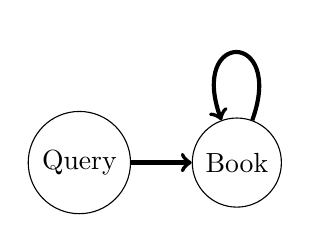
\begin{tikzpicture}
            \node[circle, draw] (n1) at (0,0) {Query};
            \node[circle, draw] (n2) at (2,0) {Book};

            \draw[->, line width=1.5pt] (n1) -- (n2);
            \draw[->, line width=1.5pt, looseness=8] (n2) to[out=70, in=110] (n2);
        \end{tikzpicture}
    \end{minipage}
    \caption{GraphQL-Schema als Graph}
\end{figure}

Generell starten alle GraphQL-Querys im Query-Type.
Erlaubte Anfragen sind dann alle Pfade mit Ursprung im Query Knoten wobei Limitierungen implementiert werden können.
Property-based Testing nimmt nun die definierten Felder im Query-Type und geht die Pfade welche sich im Graphen ergeben zufällig ab.
Nach einer bestimmten Anzahl an zufälligen Iterationen wird die Query aus dem erlangten Pfad generiert und ausgeführt.
Nutzen wir nun jedoch ein wesentlich größeres Schema, zum Beispiel die GraphQL-API von GitLab~\cite{gitlab} so erkennt man schnell, dass
der Graph so komplex wird, dass eine zufällige Pfadgenerierung zu unzuverlässig und ineffizient ist um
eine große Struktur zuverlässlich zu testen.
Einen ähnlichen Sachverhalt findet man in der Testgenerierung für Programmcode.
Dieser kann sehr komplex werden und es müssen Strategien gefunden werden um diese effizient und zuverlässlich zu testen.
Ein häufig verwendeter Ansatz ist es, den Code in einen Kontrollflussgraphen zu überführen, bei dem die Knoten Anweisungen oder Operationen darstellen
und die Kanten den möglichen Pfaden entsprechen, die während der Ausführung des Programms genommen werden können.
Hierbei wurde schon erhebliche Arbeit geleistet und diverse Kriterien entwickelt wie man eine gute Testabdeckung entwickelt.
An dieser Stelle sei insbesondere an \textit{Introduction to Software Testing}\cite{software-testing} verwiesen.
In ~\cite{software-testing} wird die Graphenüberdeckung erarbeitet und praktisch gezeigt, wie sie helfen kann um Tests zu generieren.
Es werden verschiedene Kriterien vorgestellt, die den Graphen auf unterschiedliche Art und Weise betrachten.
Wir wollen zeigen, dass das in~\cite{software-testing} erarbeitete Wissen nicht nur für Testentwicklung von Programmcode zielführend ist,
sondern auch für die Testgenerierung von anderen Graphstrukturen verwandt werden kann, in unserem Fall für die Testgenerierung für GraphQL-APIs.
Unser Fokus wird sich auf die PrimePath-Überdeckung~\cite[vgl. Criterion 2.4]{software-testing} richten da wir uns erhoffen, dass diese einen guten Mittelweg zwischen
Testgenauigkeit, Fehlerfindung und Effizienz bietet.

\section{Umsetzung}

Zuallererst wird in dieser Arbeit die grundlegende Theorie in Kapitel~\ref{theorie} definiert und in Bezug zueinander gesetzt.
Wir beginnen mit der Definition einiger Konzepte aus der Graphentheorie in Abschnitt~\ref{sec:graphentheorie}.
Darauffolgend sehen wir uns GraphQL präziser in Absatz ~\ref{graphql} an und verbinden dann beide Absätze miteinander, indem wir einen
konkreten Zusammenhang zwischen beiden Themen herstellen.
Abschließend für die grundlegende Theorie führen wir in Absatz~\ref{test} umfassend in das Thema Softwaretests ein.
Die zuvor erarbeitete Theorie wird dann im Kapitel Graphüberdeckung~\ref{graphueberdeckung} erweitert durch Theorien und Definitionen.
In diesem Kapitel zeigen wir außerdem, inwiefern die zuvor definierten Übderdeckungskriterien hinreichend für Testgenerierung für Programmcode und GraphQL sind.
Bevor wir unsere Methode entwickeln besprechen wir im Kapitel verwandte Arbeiten~\ref{relatedWork} wie der aktuelle Stand der Forschung zum Thema
automatisiertes Testen von GraphQL ist.
Mithilfe der zurvor entwickelten Theorie erarbeiten wir dann im Kapitel Testentwurf~\ref{testentwurf} ein Konzept, wie GraphQL automatisiert getestet werden kann.
Dieses Konzept wird im Kapitel~\ref{testautomatisierung} eine praktische Umsetzung in einem Prototyp finden.
Um nachzuweisen, dass der entwickelte Prototyp fähig ist, Fehler zu finden werden einige Experimente ausgeführt und mit
der \textit{Property-based} Methode~\cite{property-based-testing} verglichen im Kapitel~\ref{experimente}.
Enden wird die Arbeit mit einem kleinen Ausblick in Kapitel~\ref{futurework} und einem Fazit über unsere erreichten Verbesserungen.